\documentclass{article}

\usepackage{amsmath}
\usepackage{graphicx}

\title{My first document}
\date{2017-03-07}
\author{Minjoon Park}

\begin{document}
  \pagenumbering{gobble}
  \maketitle
  \newpage
  \tableofcontents
  \newpage
  \pagenumbering{arabic}

\section{Section}

Hello World!

\subsection{Subsection}

Structuring a document is easy!

\subsubsection{Subsubsection}

More text.

\paragraph{Paragraph}

Some more text.

\subparagraph{Subparagraph}

Even more text.

\section{Another section}

\begin{equation}
  f(x) = x^2
\end{equation}

This formula $f(x) = x^2$ is an example.

\begin{equation*}
  1 + 2 = 3
\end{equation*}

\begin{equation*}
  1 = 3 - 2
\end{equation*}

\begin{align*}
  1 + 2 &= 3\\
  1 &= 3 - 2
\end{align*}

\begin{align*}
  f(x) &= x^2\\
  g(x) &= \frac{1}{x}\\
  F(x) &= \int^a_b \frac{1}{3}x^3
\end{align*}

\begin{figure}
  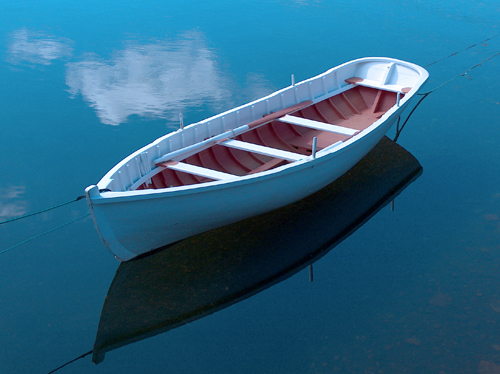
\includegraphics[width=\linewidth]{boat.jpg}
  \caption{A boat.}
  \label{fig:boat1}
\end{figure}

Figure \ref{fig:boat1} shows a boat.

Random citation \cite{DUMMY:1} embeddeed in text.

This is some example text\footnote{\label{myfootnote}Hello footnote}.

I'm referring to footnote \ref{myfootnote}.

\newpage

\bibliography{ref}
\bibliographystyle{ieeetr}

\end{document}
